\documentclass[11pt,onside,a4paper,fleqn]{report}            
\usepackage{graphicx}
\usepackage{subfigure}
\usepackage{parskip}
\usepackage{epstopdf}
\usepackage{placeins}
\usepackage{amsmath}
\usepackage{array}
\usepackage{booktabs}
\makeatletter
\renewcommand\arraystretch{2}
\renewcommand\normalsize{%
\@setfontsize\normalsize\@xpt\@xiipt
   \abovedisplayskip 4\p@ \@plus2\p@ \@minus8\p@
   \abovedisplayshortskip \z@ \@plus6\p@
   \belowdisplayshortskip 4\p@ \@plus3\p@ \@minus3\p@
   \belowdisplayskip \abovedisplayskip
   \let\@listi\@listI}
\makeatother
 
 
\parindent0pt  \parskip10pt             % make block paragraphs
                           				% do not right-justify
\title{\bf Go Language Development Trend Report}  % Supply information
\author{ \\ \\*mayuke\\}
              							%   for the title page.
\date{\today}                           %   Use current date.
 
\begin{document}                        % End of preamble, start of text.
\maketitle                              % Print title page.
\begin{abstract}

%Abstract
Golang was publicly announced in November 2009 and version 1.0 was released in March 2012. Now Go is widely used in production at Google and in many other organizations and open-source projects.In order to study the development trend of Go language in recent years, this report uses the API provided by Github to obtain a certain amount of repositories information from Github and show the development and changes of Go language from its birth to the present from several different perspectives.

\end{abstract}
\pagenumbering{roman}                   % roman page number for toc
\setcounter{page}{1}                    % make it start with "1"
\pagenumbering{arabic}					% Start text with arabic 1
\chapter{Introduction}
This report shows the development trend of Go from three different perspectives:
\begin{itemize}
\item Nearly 1,000 Github repositories are randomly selected each year from 2009 to 2021, and the number of repositories using Go is analyzed to reflect the change of popluarity of Go language.

\item The repositories built by Go language during the five years from 2017 to 2021 are selected, and the commit information of each repositories is obtained and made into a calendar 
heat map to reflect the changes in Go language user activity.

\item Crawl all description information of the repositories obtained during the five years from 2017 to 2021 and make into wordcloud map after word segmentation, so as to analyze
 the change of keywords of Go language in different years.
\end{itemize}

%\section{Objective}
 
\chapter{Implemention}

\section{The number of repositories changes over time}
\paragraph{} The change of the popularity of Go language over time can be reflected from one aspect by studying the change of the number of repositories using Go language over time. Based on this, the project uses Simple random sampling method to randomly select a certain number of repositories from Github every year and count the number of Go language repositories.

\subsection{raw data}
\paragraph{} The project uses the Github API to acquire approximately 1,200 repositories per year from 2009 to 2021, for a total of approximately 15,000 repositories, and counts Go and three other programming languages that are currently popular which are C++, Python and Java.

\paragraph{} The data results are as follows:

% Data Table
\begin{table}[ht]
\renewcommand{\arraystretch}{1.3}
\setlength\tabcolsep{5pt}
\begin{tabular}{@{}llllllllllllll@{}}
\toprule
years  & 09 & 10 & 11 & 12 & 13 & 14 & 15 & 16 & 17 & 18 & 19 & 20 & 21 \\ \midrule
Go     & 5    & 7    & 14   & 19   & 37   & 55   & 58   & 54   & 59   & 70   & 61   & 57   & 69   \\
C++    & 32   & 45   & 68   & 65   & 75   & 61   & 65   & 66   & 52   & 68   & 53   & 71   & 48   \\
Java   & 43   & 67   & 87   & 86   & 97   & 121  & 143  & 129  & 95   & 68   & 59   & 45   & 35   \\
Python & 139  & 166  & 155  & 141  & 124  & 120  & 117  & 151  & 208  & 243  & 255  & 253  & 249  \\ \bottomrule
\end{tabular}
\caption{The number of repositories in different languages per 1000 repositories}
\end{table}

\paragraph{} This data is plotted into line chart 2.1, which visually shows how the four programming languages changed between 2009 and 2021.It is shown in the figure that the number of Go language repositories has been on the rise, which indicates that Go
languages are becoming more and more popular in recent years.

%figure 2.1
\begin{figure}[ht]
\centering
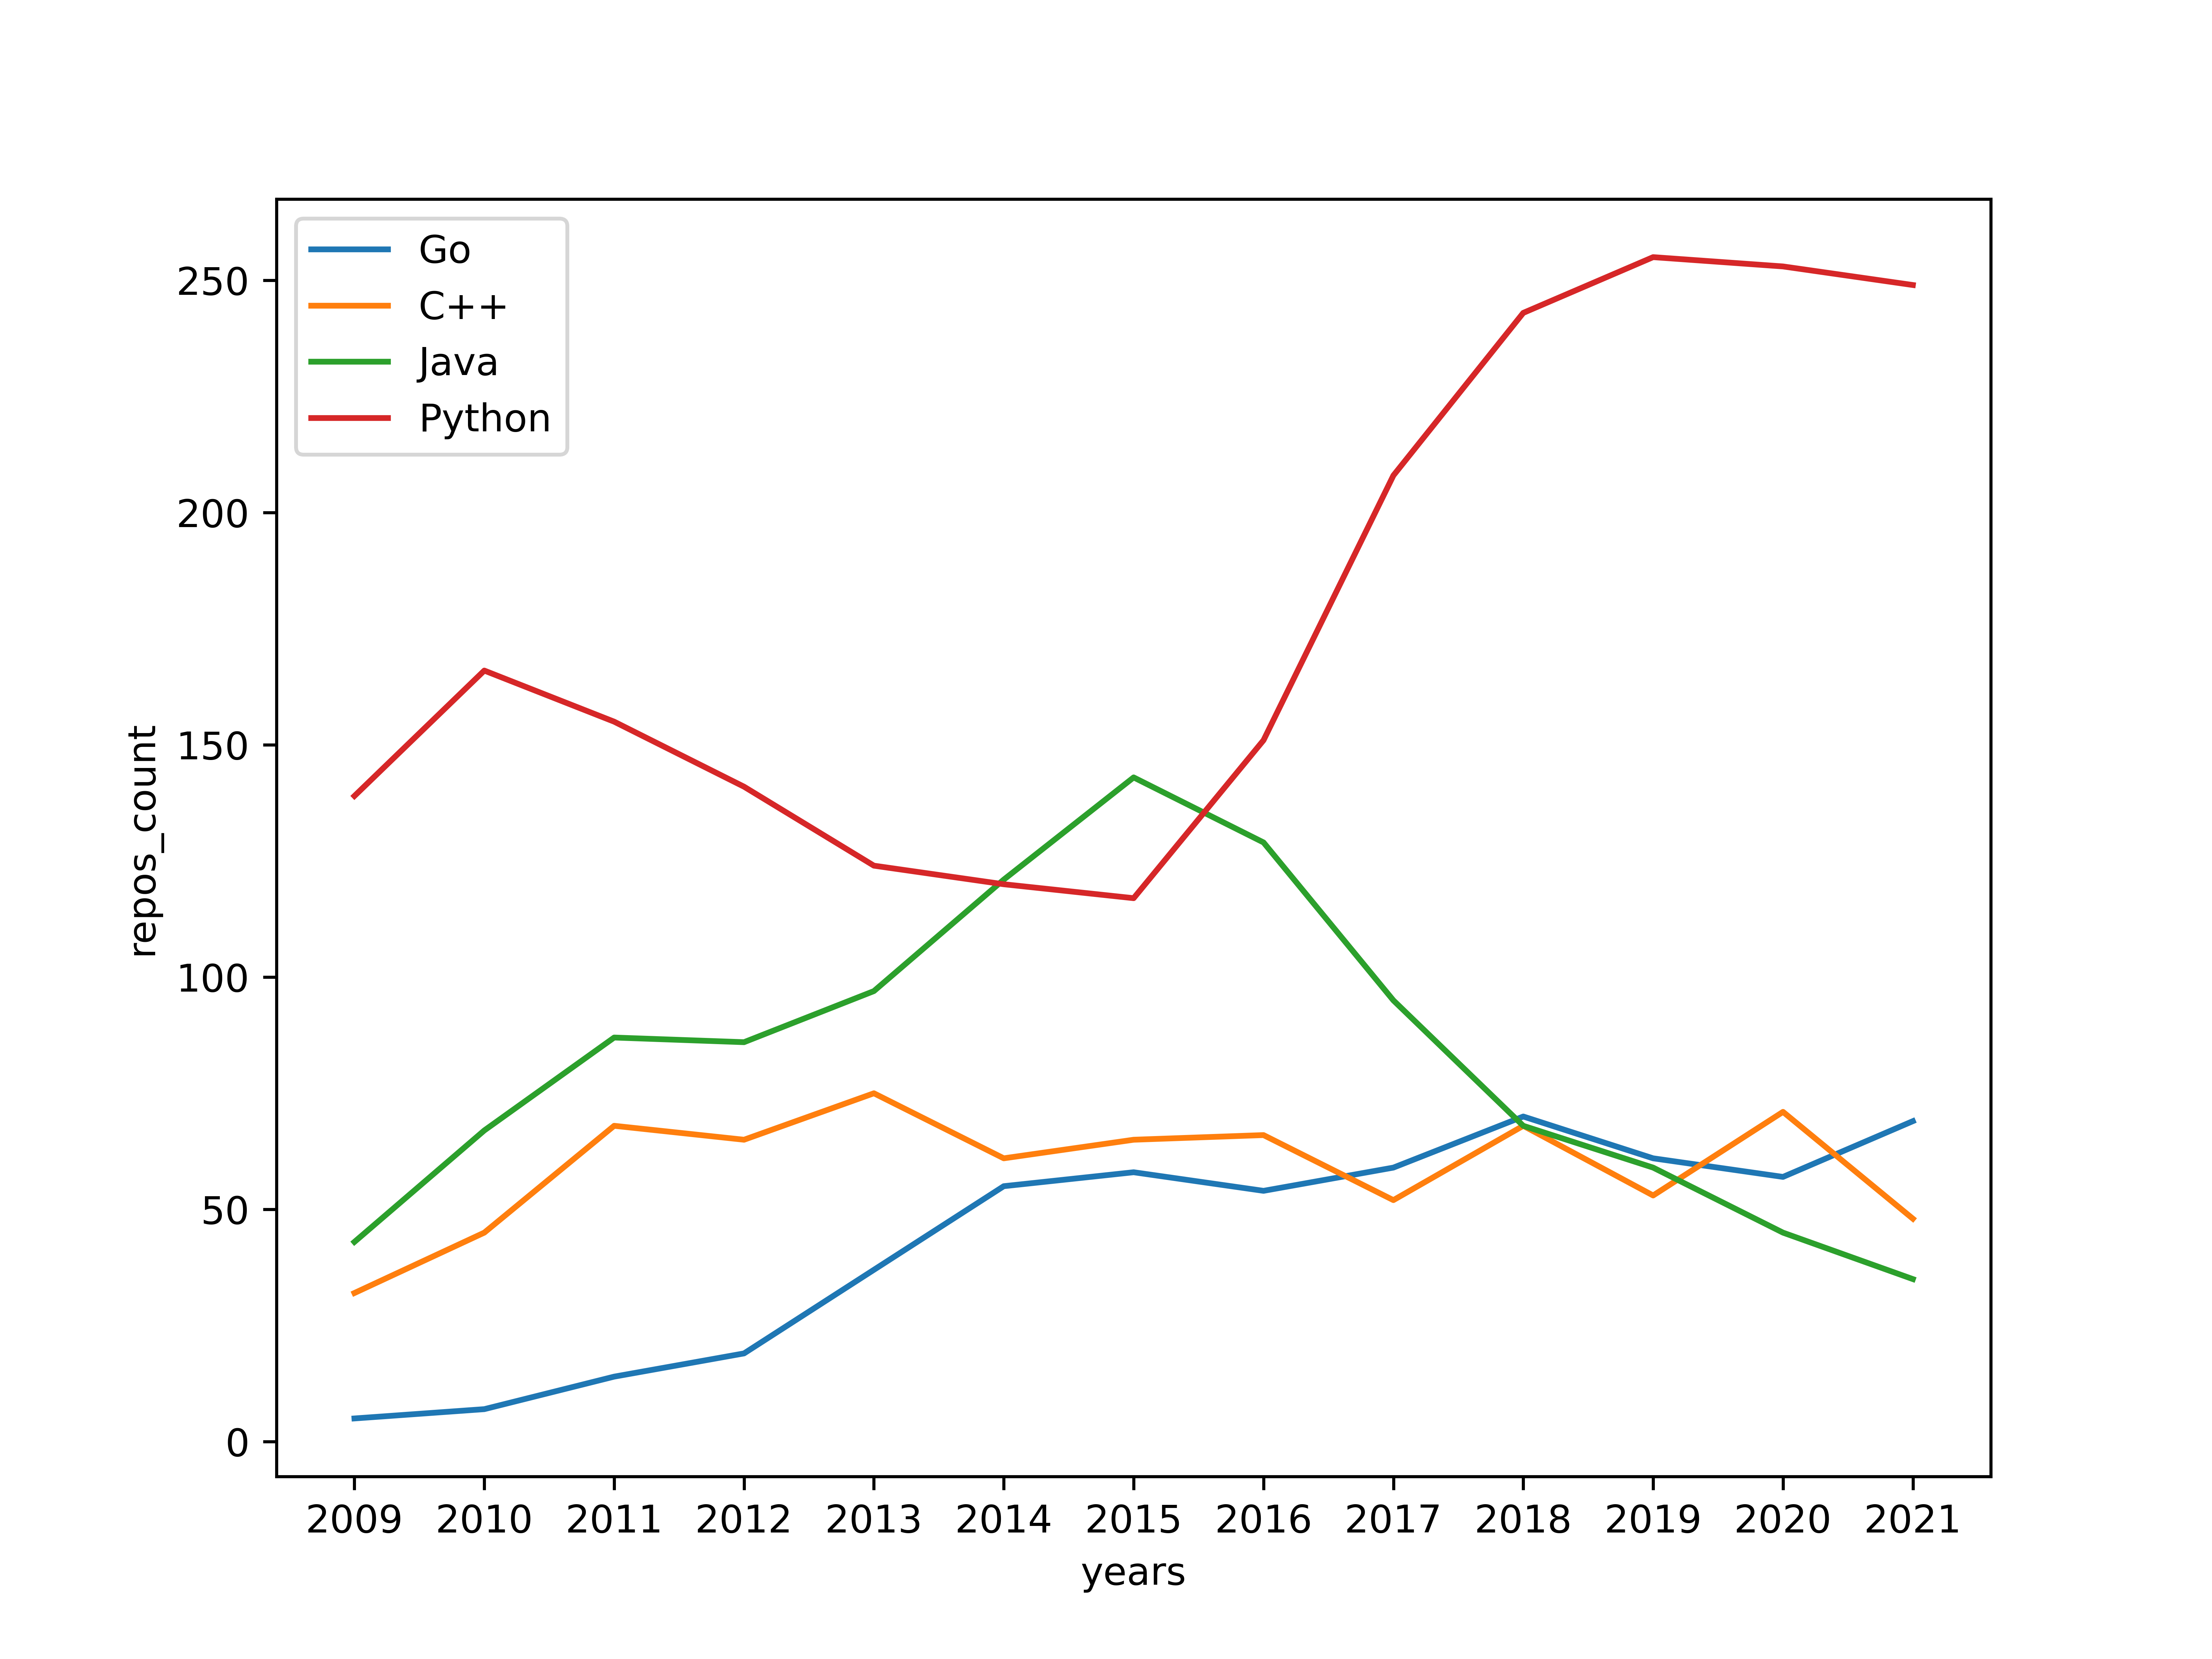
\includegraphics[scale=0.6]{result/yearsChange.png}
\caption{The number of repositories varies by programming language}
\label{fig:pathdemo4}
\end{figure}

\subsection{Redefination of Popularity of Programing language}
\paragraph{} Intuitively, the number of repositories is not the only indicator of language popularity. There are several
other important indicators that can be used to reflect the popularity of a repositories in the extracted
Github repositories information. To better introduce these indicators, let's first understand some concepts
related to them. These concepts are limited to the Github platform.

\paragraph{stars} You can star repositories and topics to keep track of projects you find interesting and discover related 
content in your news feed. Starring makes it easy to find a repository or topic again later. Starring a repository 
also shows appreciation to the repository maintainer for their work. Many of GitHub's repository rankings 
depend on the number of stars a repository has. In addition, Github Explore shows popular repositories based 
on the number of stars they have.

\paragraph{watch} You can watch a repository to receive notifications for new pull requests and issues. When the owner 
updates the repository, you'll see the changes in your personal dashboard.

\paragraph{fork} A fork is a copy of a repository. Forking a repository allows you to freely experiment with changes 
without affecting the original project.

\paragraph{} Based on these concepts, we can redefine the popularity of a repository as \textbf{\emph{Hot}}, expressed by formula 2-1:

 $$Hot = repos * (log(stars) + log(watch) + forks)$$

\paragraph{} After crawling the data required by the formula and calculating the Hot value, the data for each programming language is tabulated below.

\begin{table}[ht]
\renewcommand{\arraystretch}{1} % Default value: 1
\begin{tabular}{@{}llllll@{}}
\toprule
years & repos\_count & stargazers\_count & watchers\_count & forks\_count & hot     \\ \midrule
2009  & 5            & 105               & 105             & 17           & 87.58   \\
2010  & 7            & 257               & 257             & 41           & 149.58  \\
2011  & 14           & 1412              & 1412            & 287          & 407.29  \\
2012  & 19           & 3435              & 3435            & 899          & 632.78  \\
2013  & 37           & 10106             & 10106           & 1787         & 1384.14 \\
2014  & 55           & 18936             & 18936           & 2894         & 2195.41 \\
2015  & 58           & 25211             & 25211           & 4159         & 2393.40 \\
2016  & 54           & 26055             & 26055           & 3950         & 2229.45 \\
2017  & 59           & 27661             & 27661           & 6941         & 2494.05 \\
2018  & 70           & 27107             & 27107           & 5161         & 2925.03 \\
2019  & 61           & 19269             & 19269           & 3445         & 2453.31 \\
2020  & 57           & 15722             & 15722           & 2552         & 2234.31 \\
2021  & 69           & 8196              & 8196            & 1173         & 2497.62 \\ \bottomrule
\end{tabular}
\caption{Go language data}

\renewcommand{\arraystretch}{1} % Default value: 1
\begin{tabular}{@{}llllll@{}}
\toprule
years & repos\_count & stargazers\_count & watchers\_count & forks\_count & hot     \\ \midrule
2009  & 32           & 491               & 491             & 282          & 832.60  \\
2010  & 45           & 1729              & 1729            & 1103         & 1422.84 \\
2011  & 68           & 6631              & 6631            & 2735         & 2502.90 \\
2012  & 65           & 11438             & 11438           & 4905         & 2549.50 \\
2013  & 75           & 20085             & 20085           & 6956         & 3101.38 \\
2014  & 61           & 20841             & 20841           & 7526         & 2535.89 \\
2015  & 65           & 29471             & 29471           & 7543         & 2767.37 \\
2016  & 66           & 31531             & 31531           & 9768         & 2847.43 \\
2017  & 52           & 24563             & 24563           & 6377         & 2173.97 \\
2018  & 68           & 26508             & 26508           & 6907         & 2865.66 \\
2019  & 53           & 17151             & 17151           & 3739         & 2120.02 \\
2020  & 71           & 18167             & 18167           & 4366         & 2867.70 \\
2021  & 48           & 5897              & 5897            & 1138         & 1689.78 \\ \bottomrule
\end{tabular}
\caption{C++ language data}
\end{table}

\begin{table}[ht]
\renewcommand{\arraystretch}{1} % Default value: 1
\begin{tabular}{@{}llllll@{}}
\toprule
years & repos\_count & stargazers\_count & watchers\_count & forks\_count & hot     \\ \midrule
2009  & 43           & 660               & 660             & 905          & 1227.84 \\
2010  & 67           & 2679              & 2679            & 1843         & 2252.73 \\
2011  & 87           & 8531              & 8531            & 5289         & 3348.26 \\
2012  & 86           & 14999             & 14999           & 7933         & 3500.10 \\
2013  & 97           & 25975             & 25975           & 10764        & 4144.19 \\
2014  & 121          & 41429             & 41429           & 15500        & 5396.20 \\
2015  & 143          & 66296             & 66296           & 24079        & 6662.19 \\
2016  & 129          & 62046             & 62046           & 19609        & 5947.07 \\
2017  & 95           & 44474             & 44474           & 24969        & 4321.47 \\
2018  & 68           & 26958             & 26958           & 10045        & 2905.71 \\
2019  & 59           & 18991             & 18991           & 5171         & 2404.97 \\
2020  & 45           & 11381             & 11381           & 2886         & 1729.96 \\
2021  & 35           & 4295              & 4295            & 1484         & 1213.53 \\ \bottomrule
\end{tabular}
\caption{Java language data}

\renewcommand{\arraystretch}{1} % Default value: 1
\begin{tabular}{@{}llllll@{}}
\toprule
years & repos\_count & stargazers\_count & watchers\_count & forks\_count & hot      \\ \midrule
2009  & 139          & 2054              & 2054            & 659          & 4360.79  \\
2010  & 166          & 6468              & 6468            & 1878         & 6008.07  \\
2011  & 155          & 14898             & 14898           & 5582         & 6226.70  \\
2012  & 141          & 24205             & 24205           & 8894         & 5956.50  \\
2013  & 124          & 32898             & 32898           & 9180         & 5353.79  \\
2014  & 120          & 40846             & 40846           & 12527        & 5309.83  \\
2015  & 117          & 53848             & 53848           & 16294        & 5314.76  \\
2016  & 151          & 72494             & 72494           & 20916        & 7043.16  \\
2017  & 208          & 98002             & 98002           & 28227        & 9972.73  \\
2018  & 243          & 94256             & 94256           & 24024        & 11566.99 \\
2019  & 255          & 82564             & 82564           & 19163        & 11957.58 \\
2020  & 253          & 64301             & 64301           & 15533        & 11604.64 \\
2021  & 249          & 30126             & 30126           & 9814         & 10711.50 \\ \bottomrule
\end{tabular}
\caption{Python language data}
\end{table}

\paragraph{} The modified line graph is shown in Figure. 2.2. Compared with Figure. 2.1, except for the changes in the ordinate
value, the monotonicity of the curve hardly changes much. As is shown in the picture, from 2009 to 2021, the popularity of Go language has been rising steadily.

%figure 2.2
\begin{figure}[ht]
\centering
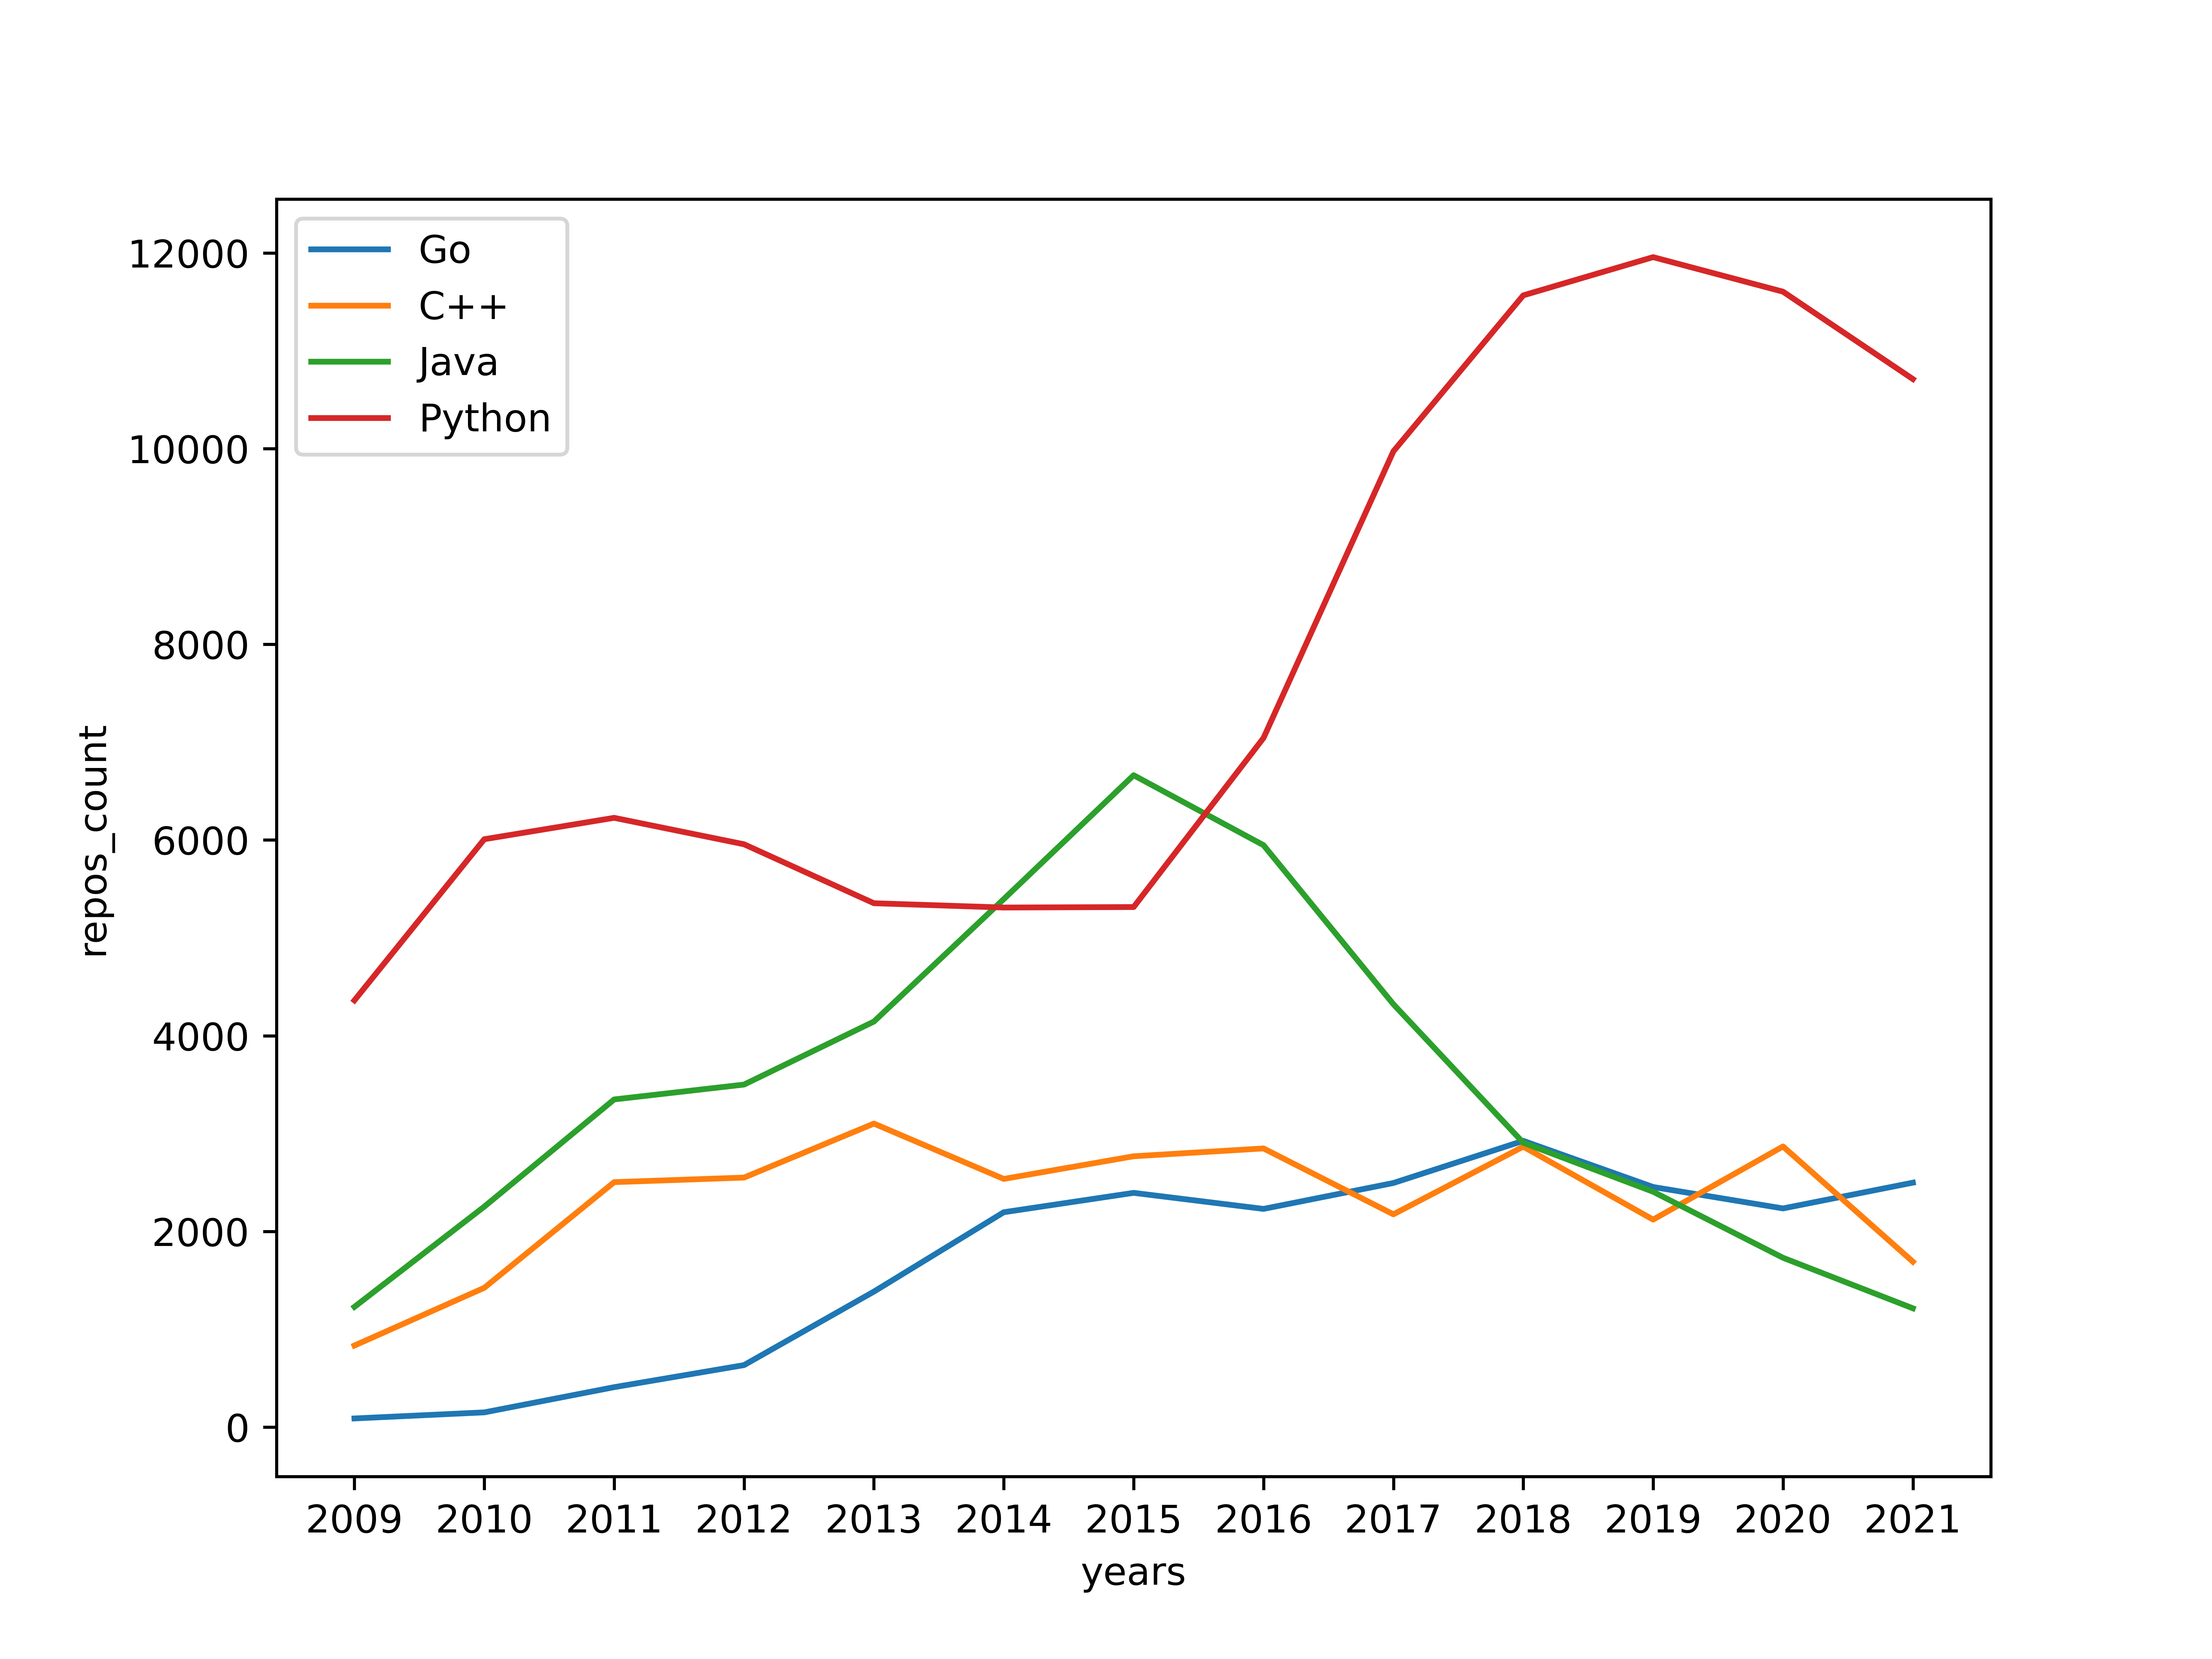
\includegraphics[scale=0.6]{result/yearsChange_modifed.png}
\caption{Programming language popularity changes over time}
\label{fig:pathdemo4}
\end{figure}

\section{Changes in developer activity}
\paragraph{} Another way to measure the popularity of a programming language is to analyze the level of activity among
developers who use that language. Github is a distributed code hosting platform based on Git. In the version 
control tool Git,git-commit records the changes made to the repository by the developer, including the changes and change time made to the project.

\paragraph{} This project extracted nearly 10,000 Git repositories built using Go over the past five years and obtained all
their commit information, totaling 200,000. The commit time information is then extracted and turned into
a calendar heat map to analyze the changes in Go developer activity.

\begin{figure}[]
\centering
\includegraphics[scale=0.4]{result/commits.png}
\caption{Programming language popularity changes over time}
\label{fig:pathdemo4}
\end{figure}

\paragraph{} As we can see in the calendar images Figure2.3, the colors on the calendar have deepened from 2017 to 2022, representing more and more development activity using the Go language

\section{Go language word cloud}

\paragraph{} As we all know, each programming language has its own unique characteristics, and one way to understand 
the characteristics of Go is to gather a lot of information about it and find out what the key information is. 
Wordcloud pictures are an appropriate approach.


\paragraph{} For each Github repository that we crawled using the Go language, we used Github's API to get the description 
of the repository, and then summarized the information and saved it in a file. Finally made it into a word cloud map.

\begin{figure}[]
\subfigure[2017]
{
    \begin{minipage}[]{.4\linewidth}
        \centering
        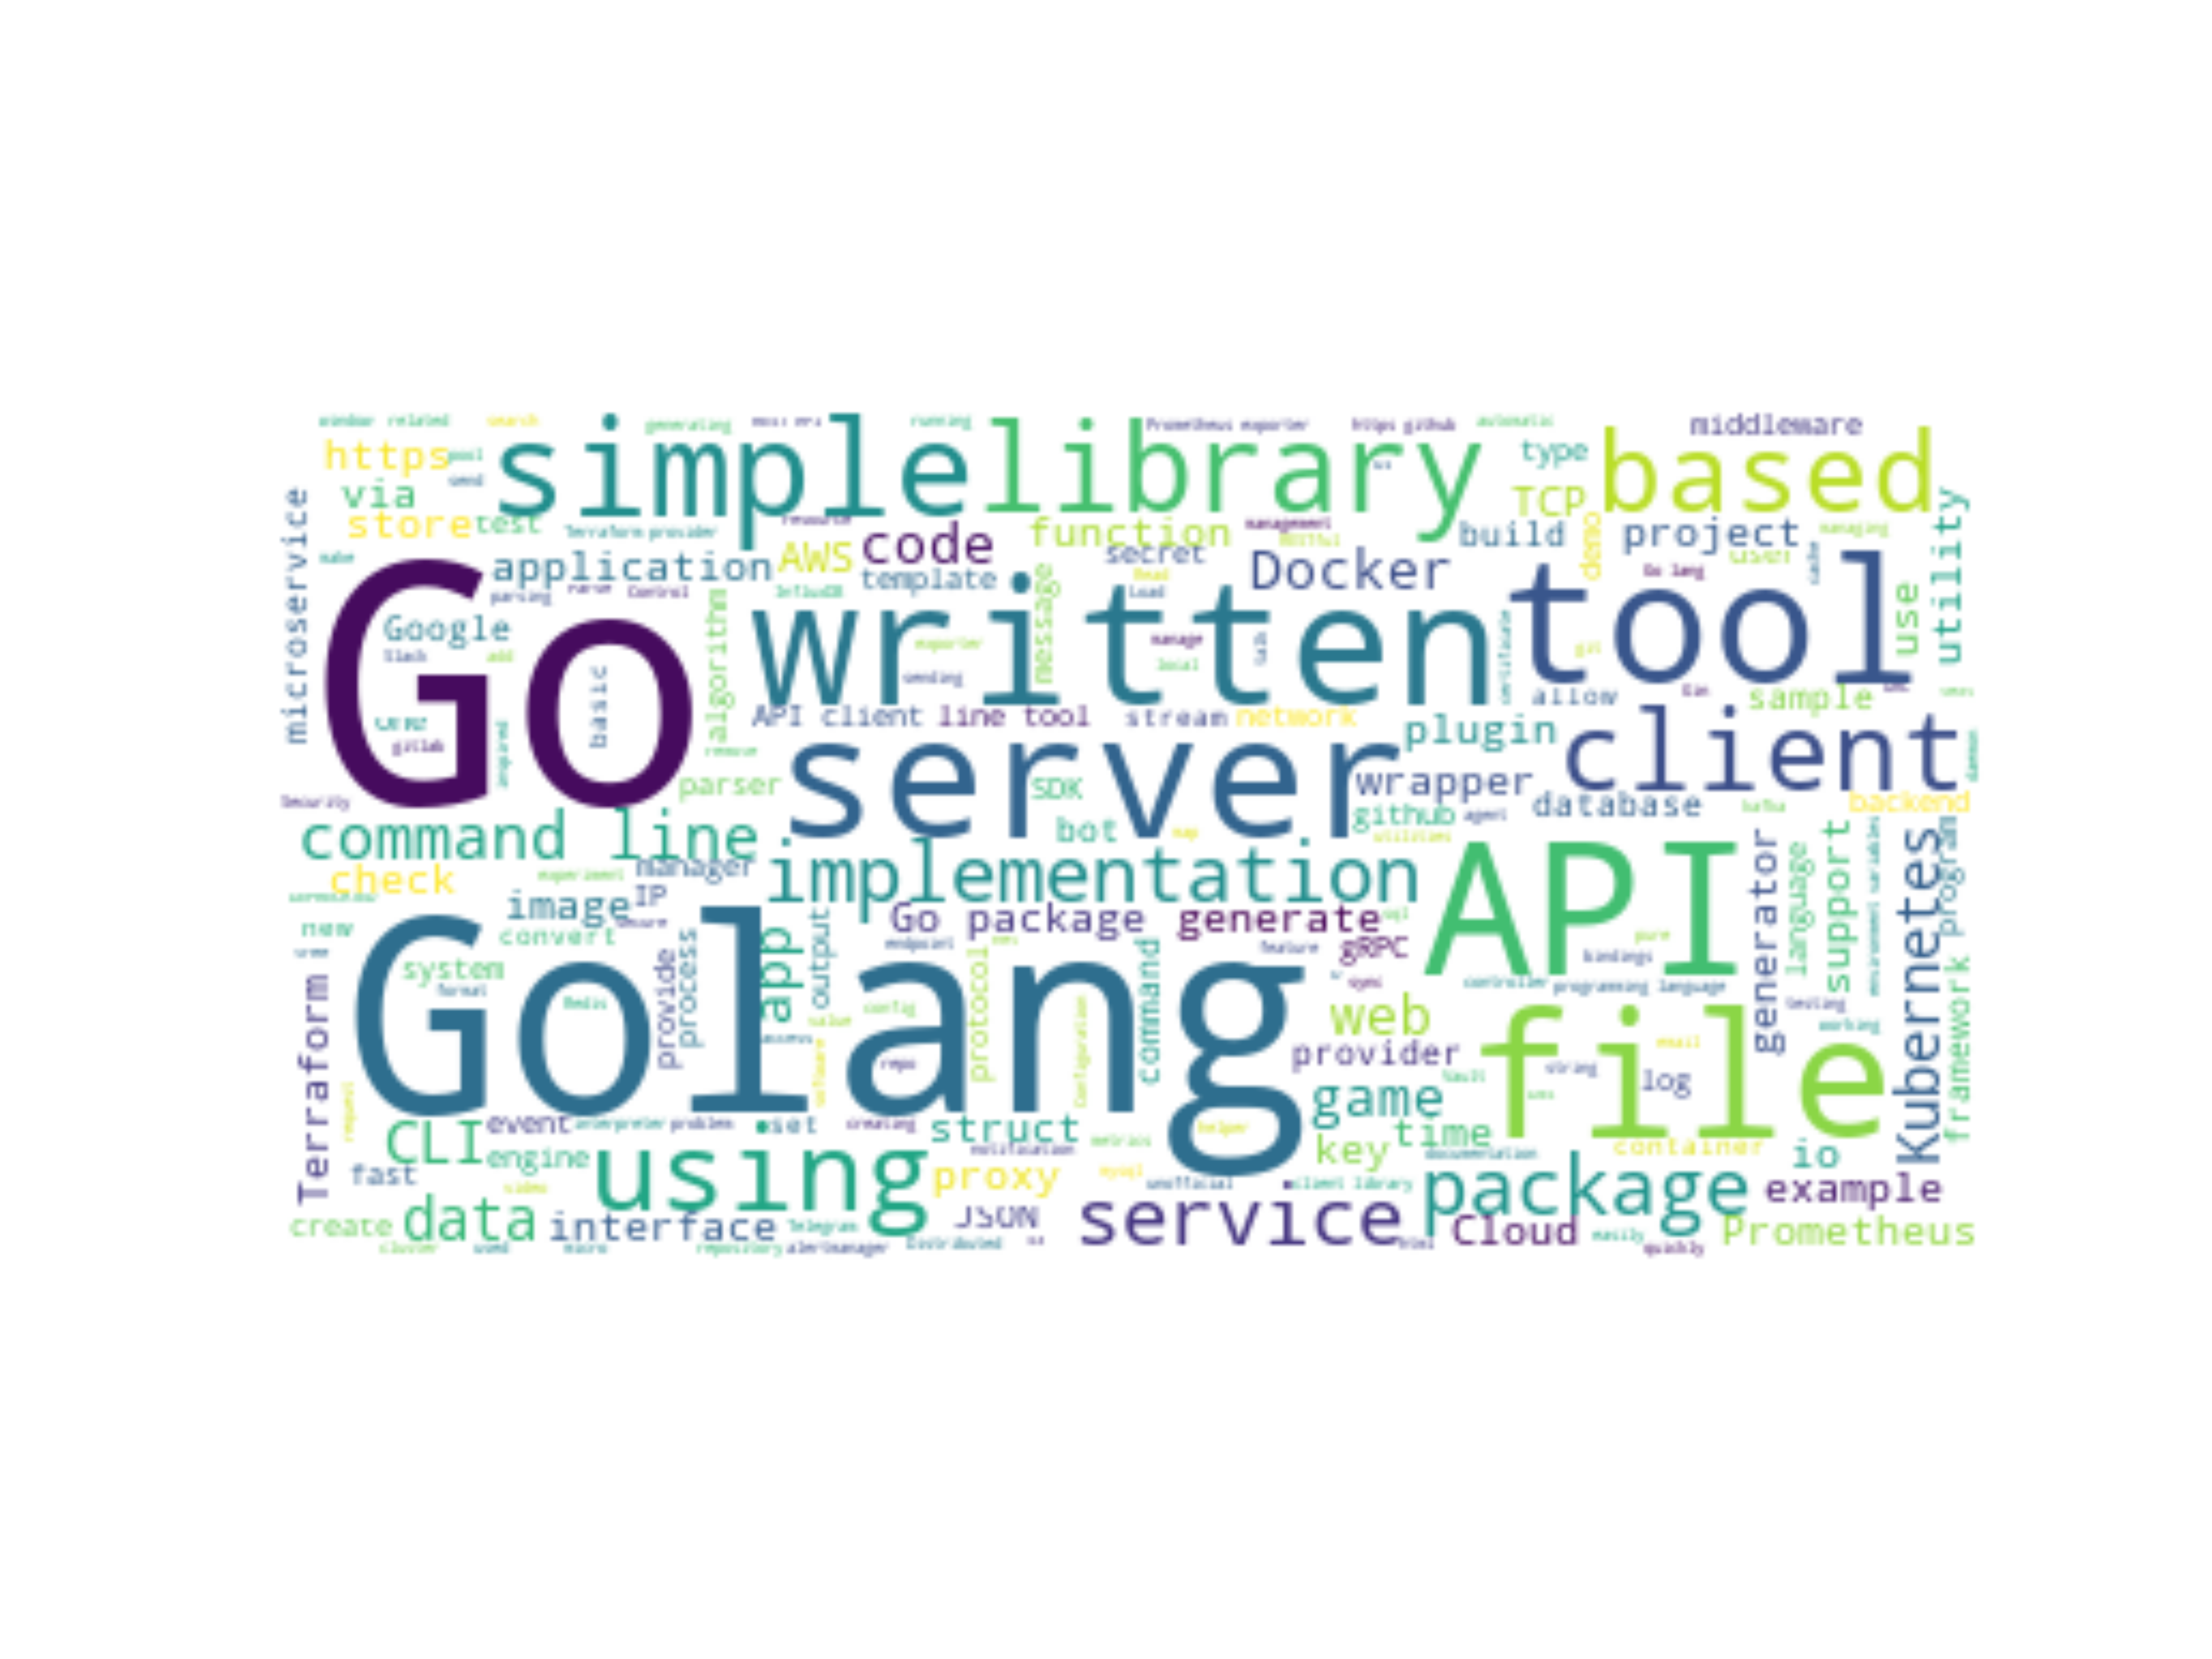
\includegraphics[scale=0.4]{result/2017.dat.png}
    \end{minipage}
}
\subfigure[2018]
{
 	\begin{minipage}[]{.4\linewidth}
        \centering
        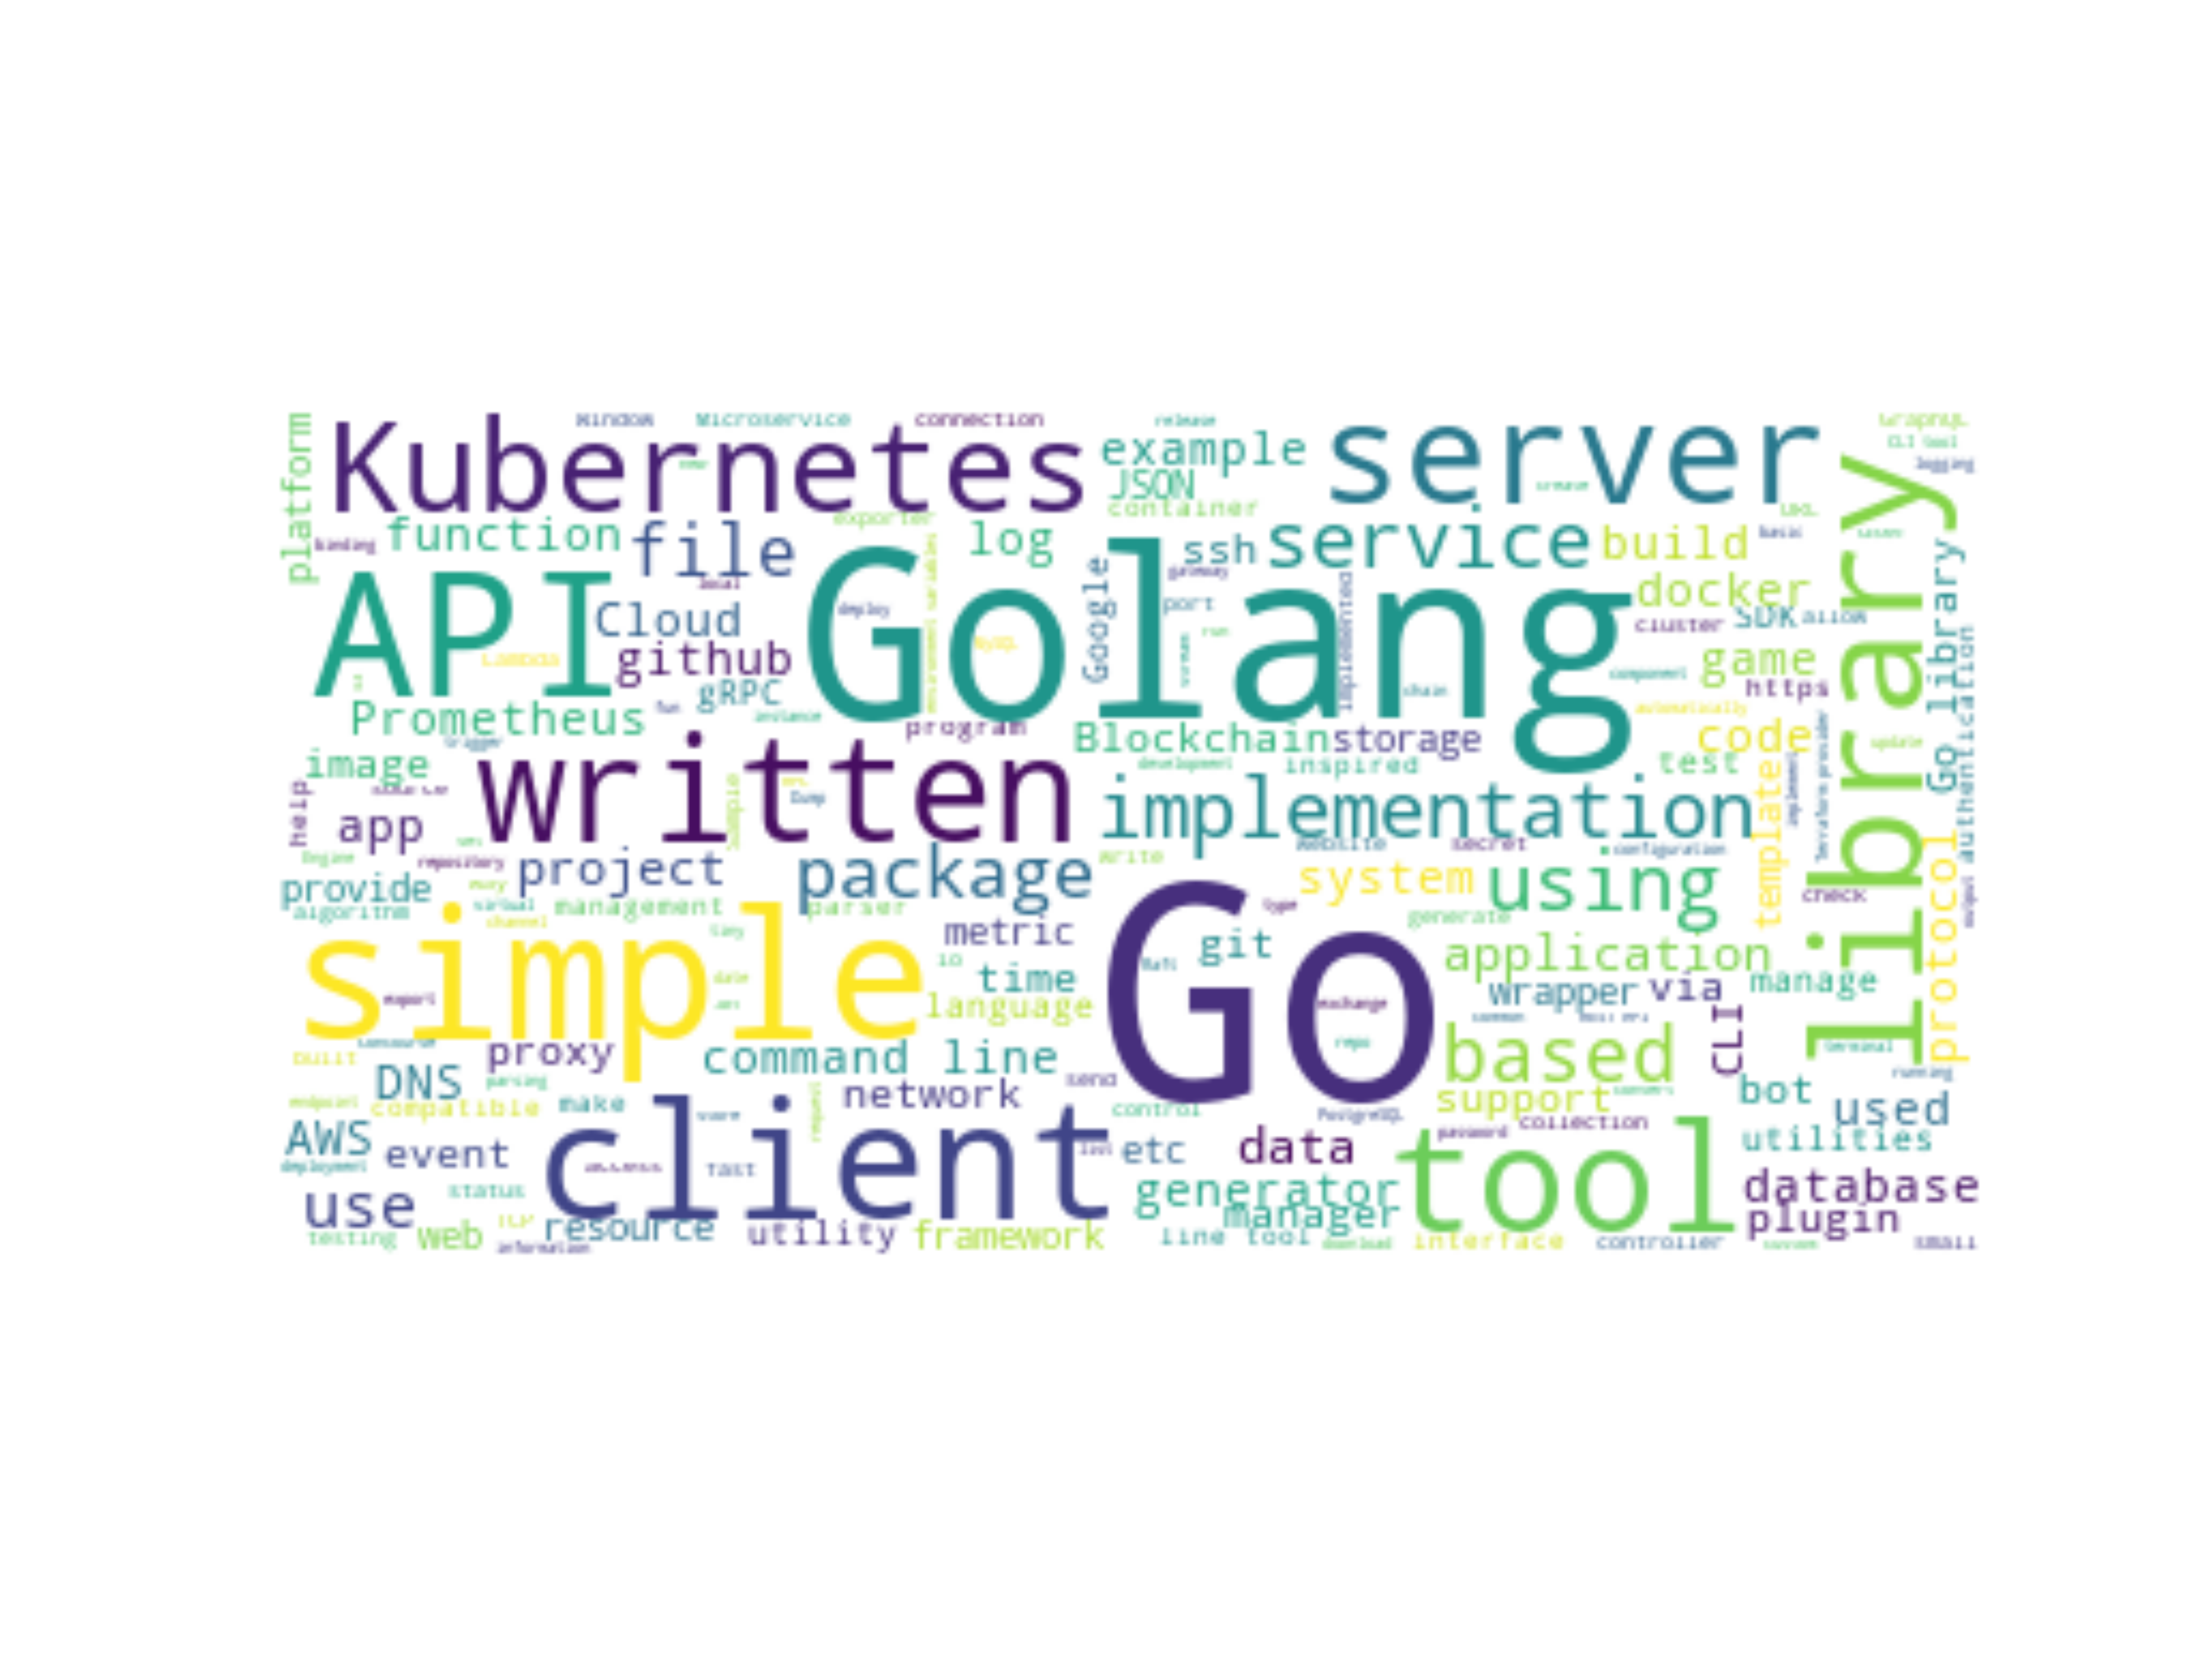
\includegraphics[scale=0.4]{result/2018.dat.png}
    \end{minipage}
}
\subfigure[2019]
{
 	\begin{minipage}[]{.4\linewidth}
        \centering
        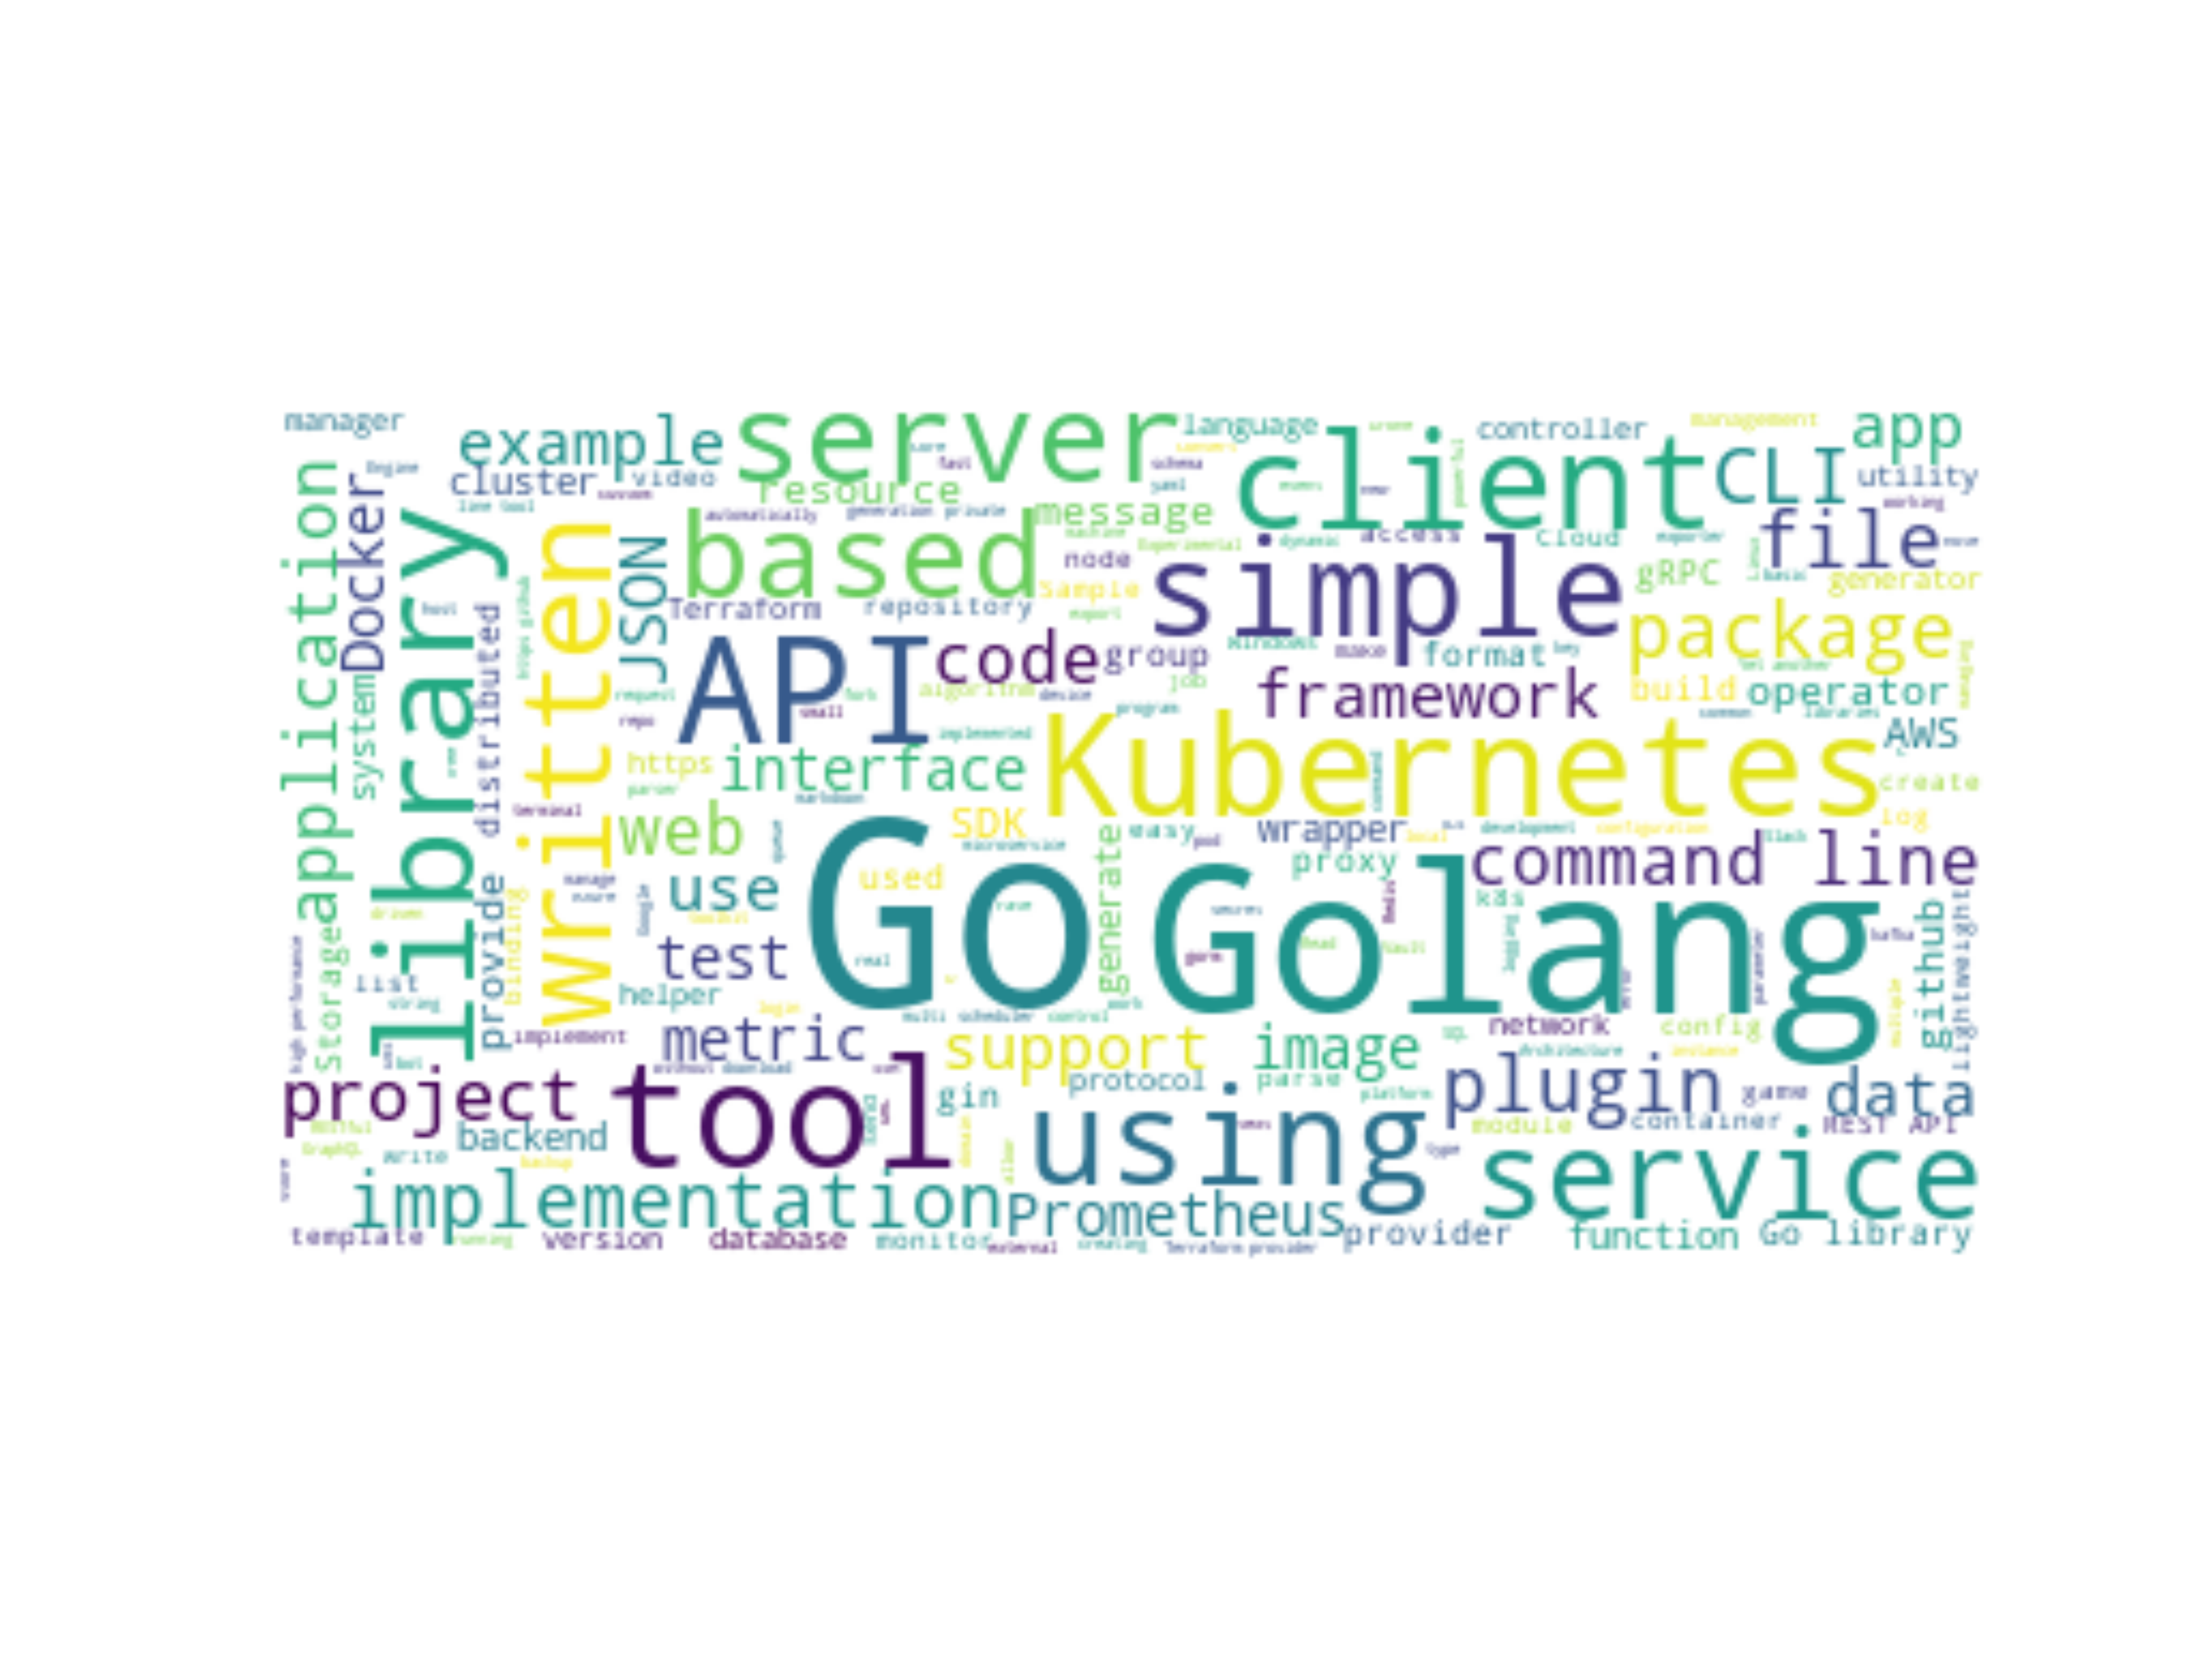
\includegraphics[scale=0.4]{result/2019.dat.png}
    \end{minipage}
}
\subfigure[2020]
{
 	\begin{minipage}[]{.4\linewidth}
        \centering
        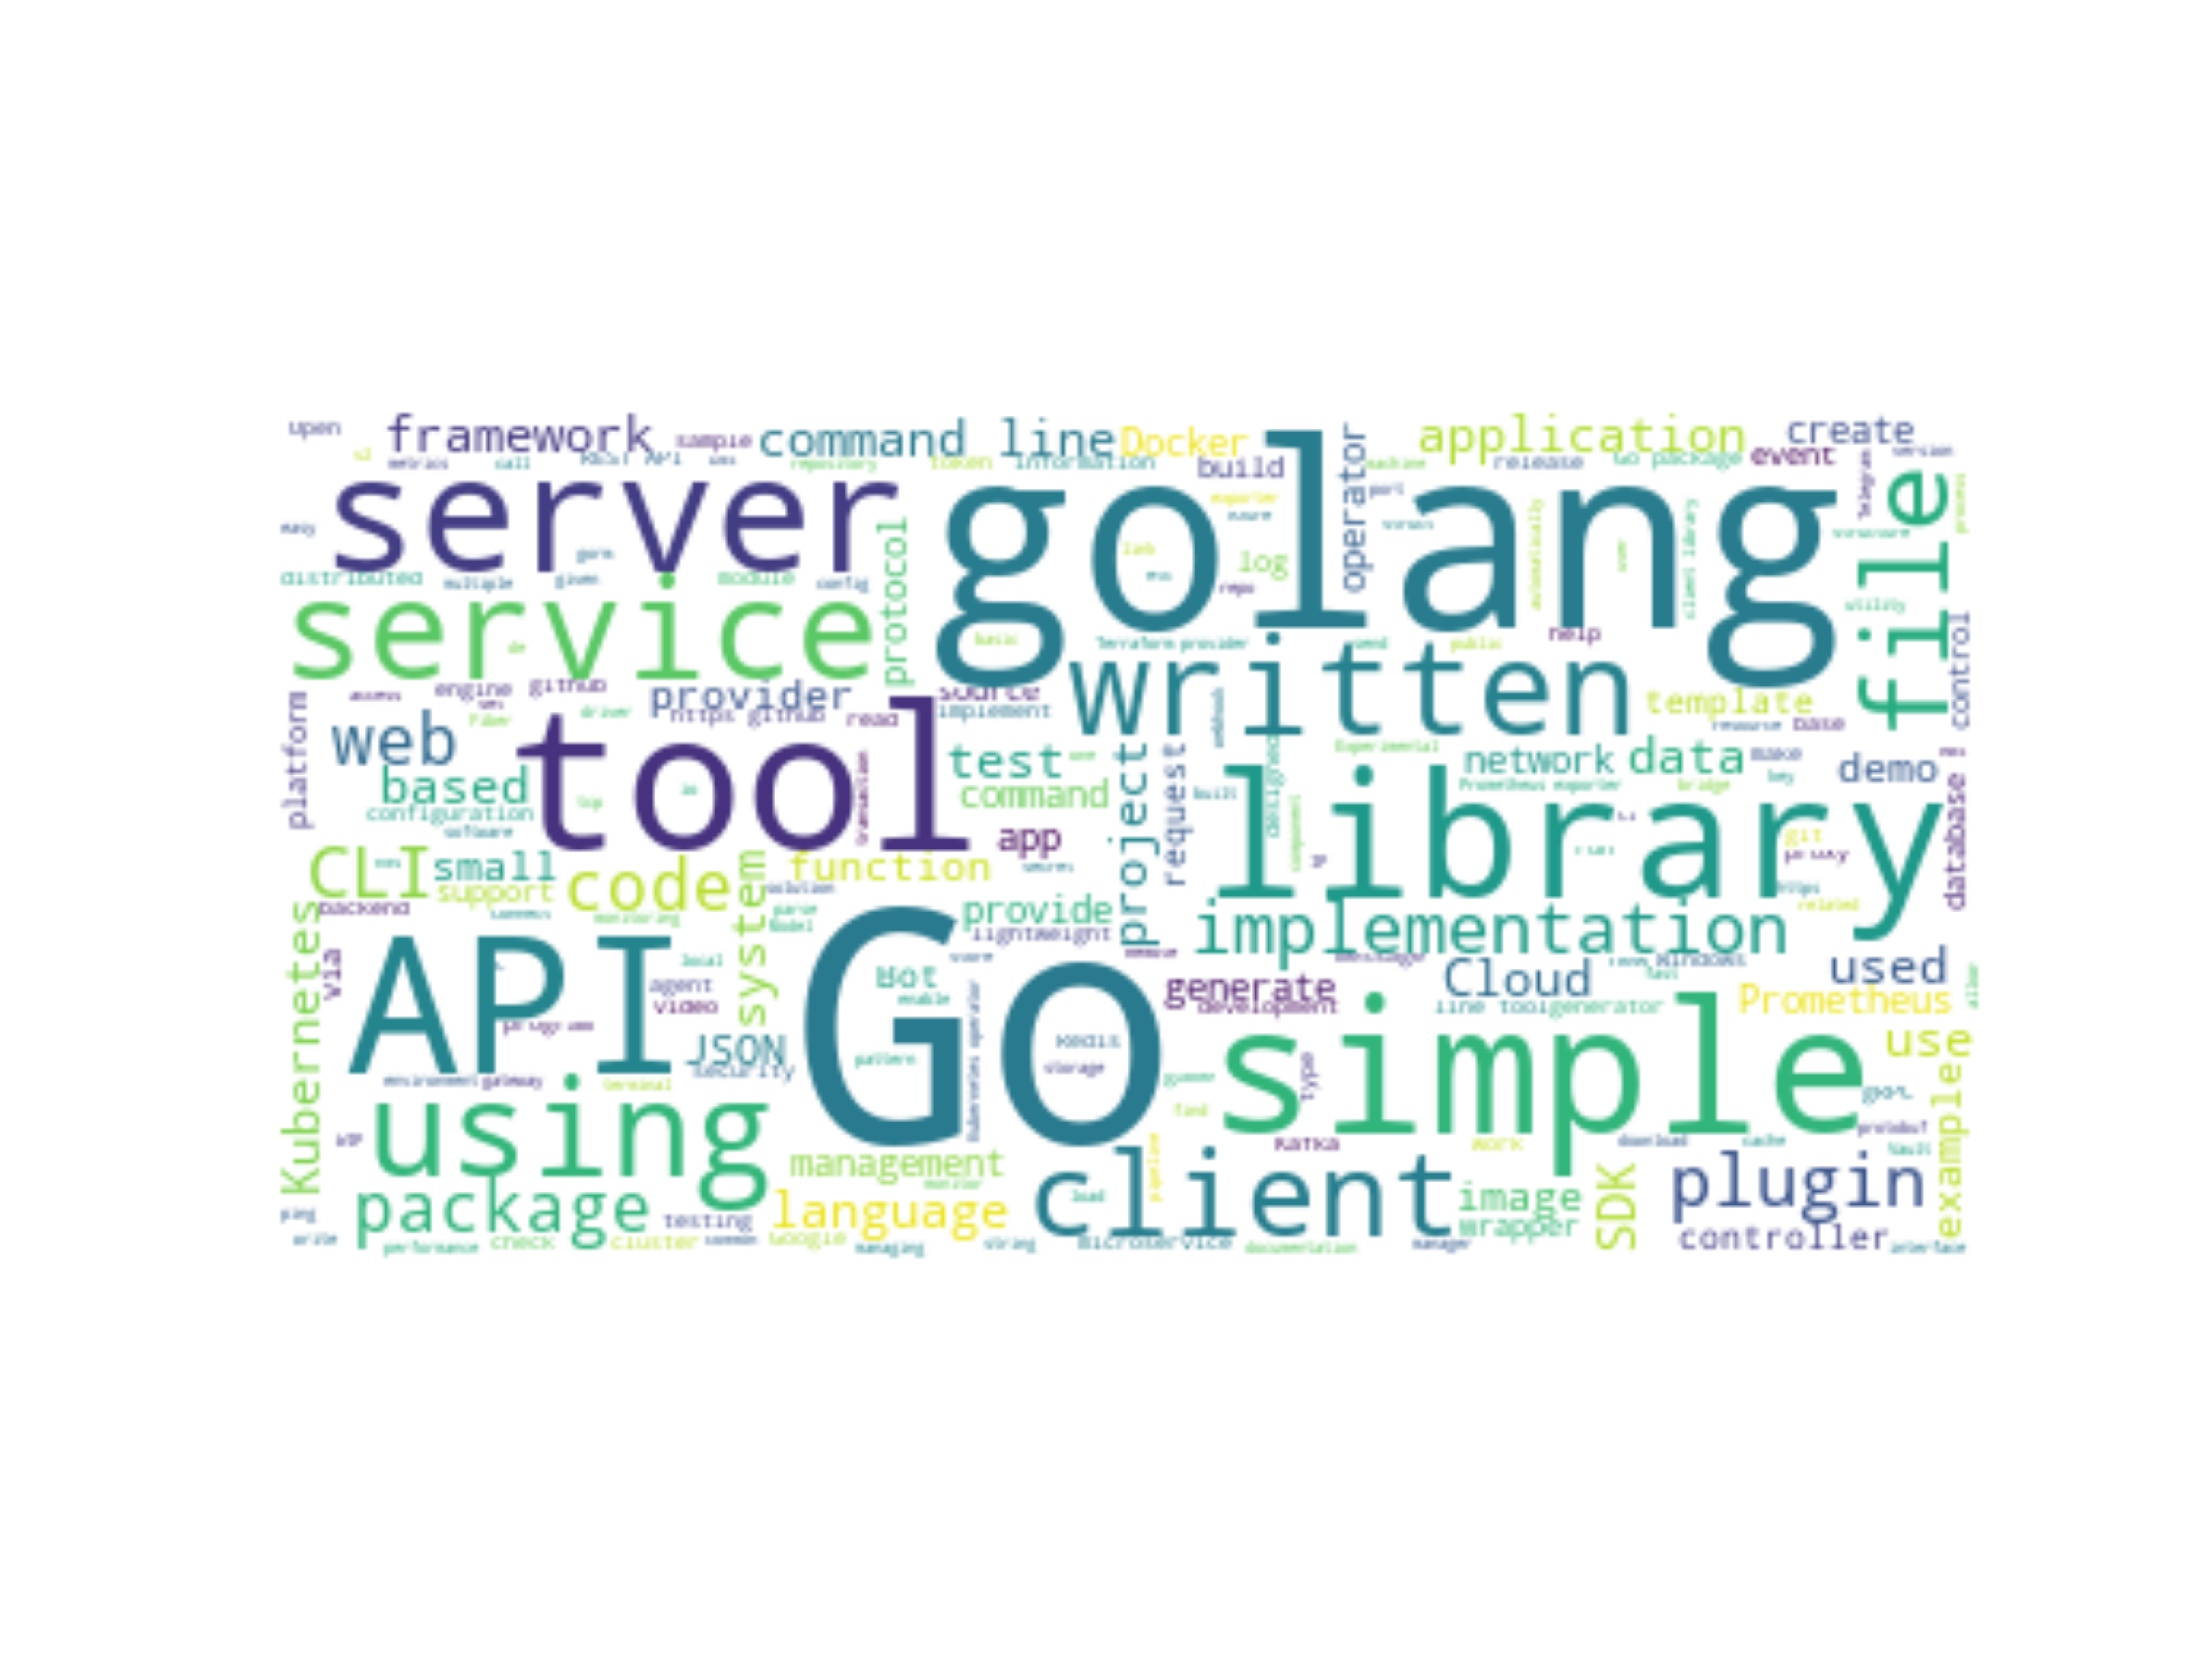
\includegraphics[scale=0.4]{result/2020.dat.png}
    \end{minipage}
}
\subfigure[2021]
{
 	\begin{minipage}[]{.4\linewidth}
        \centering
        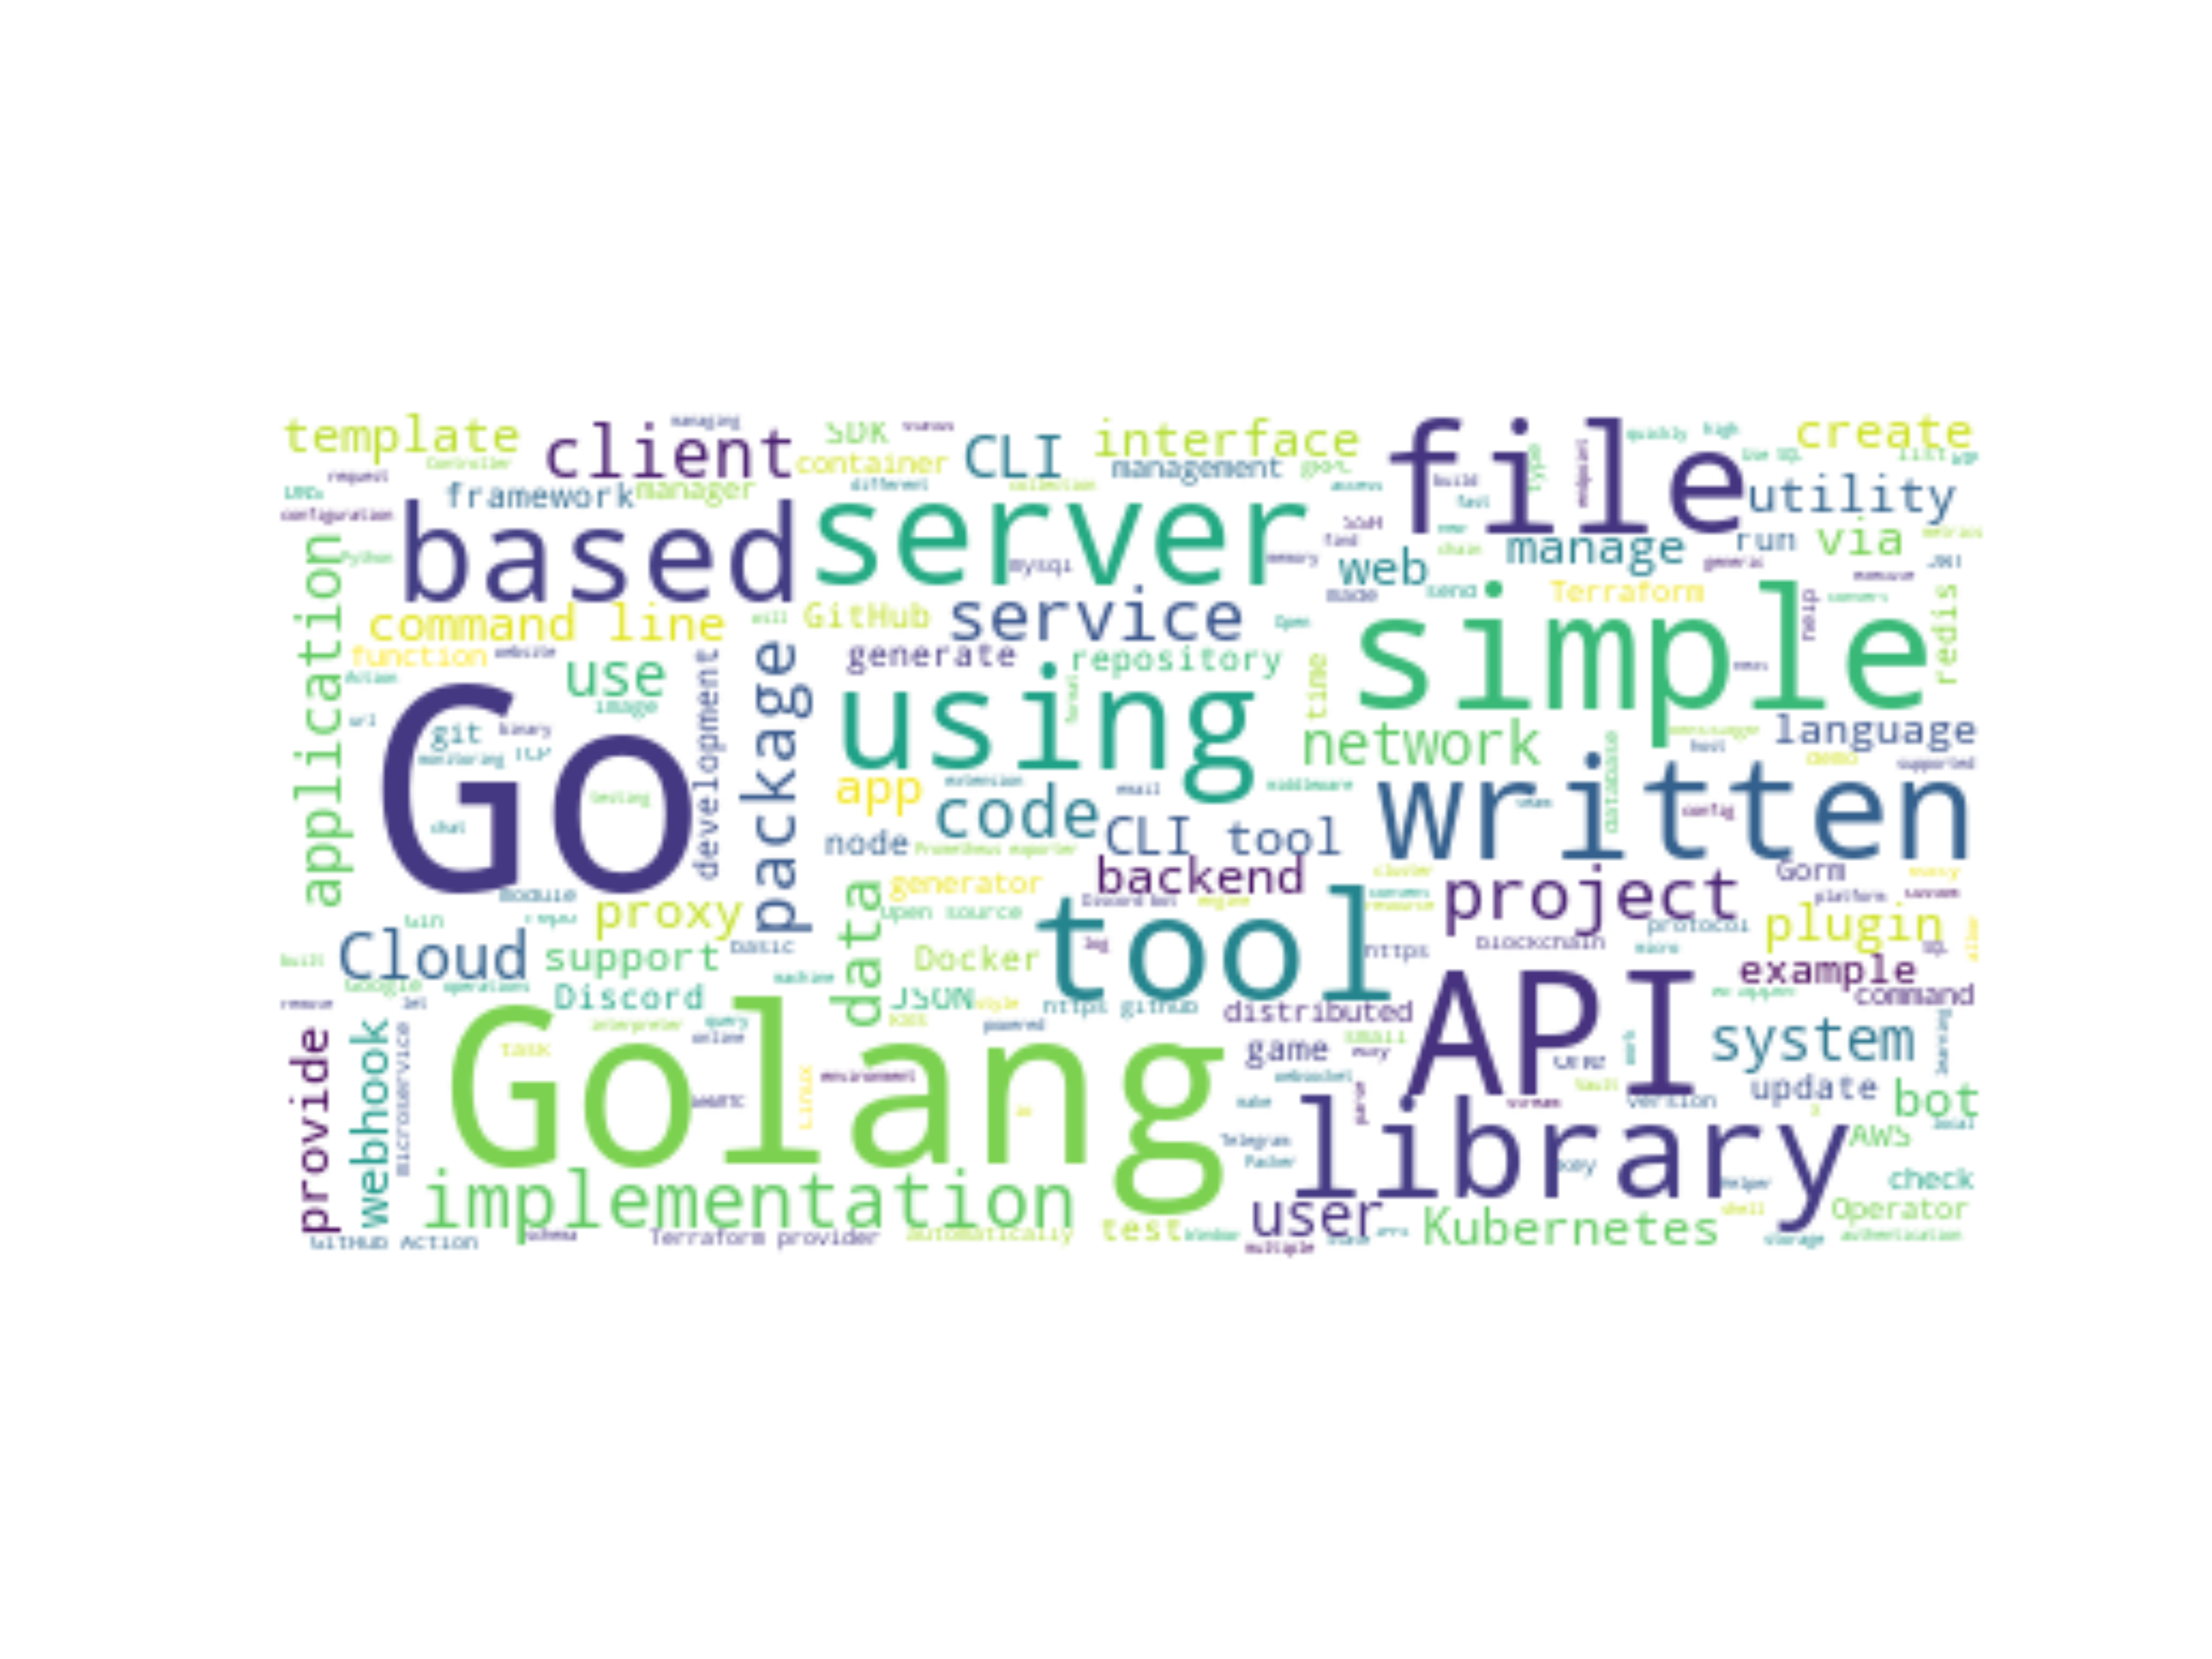
\includegraphics[scale=0.4]{result/2021.dat.png}
    \end{minipage}
}
\subfigure[all]
{
 	\begin{minipage}[]{.4\linewidth}
        \centering
        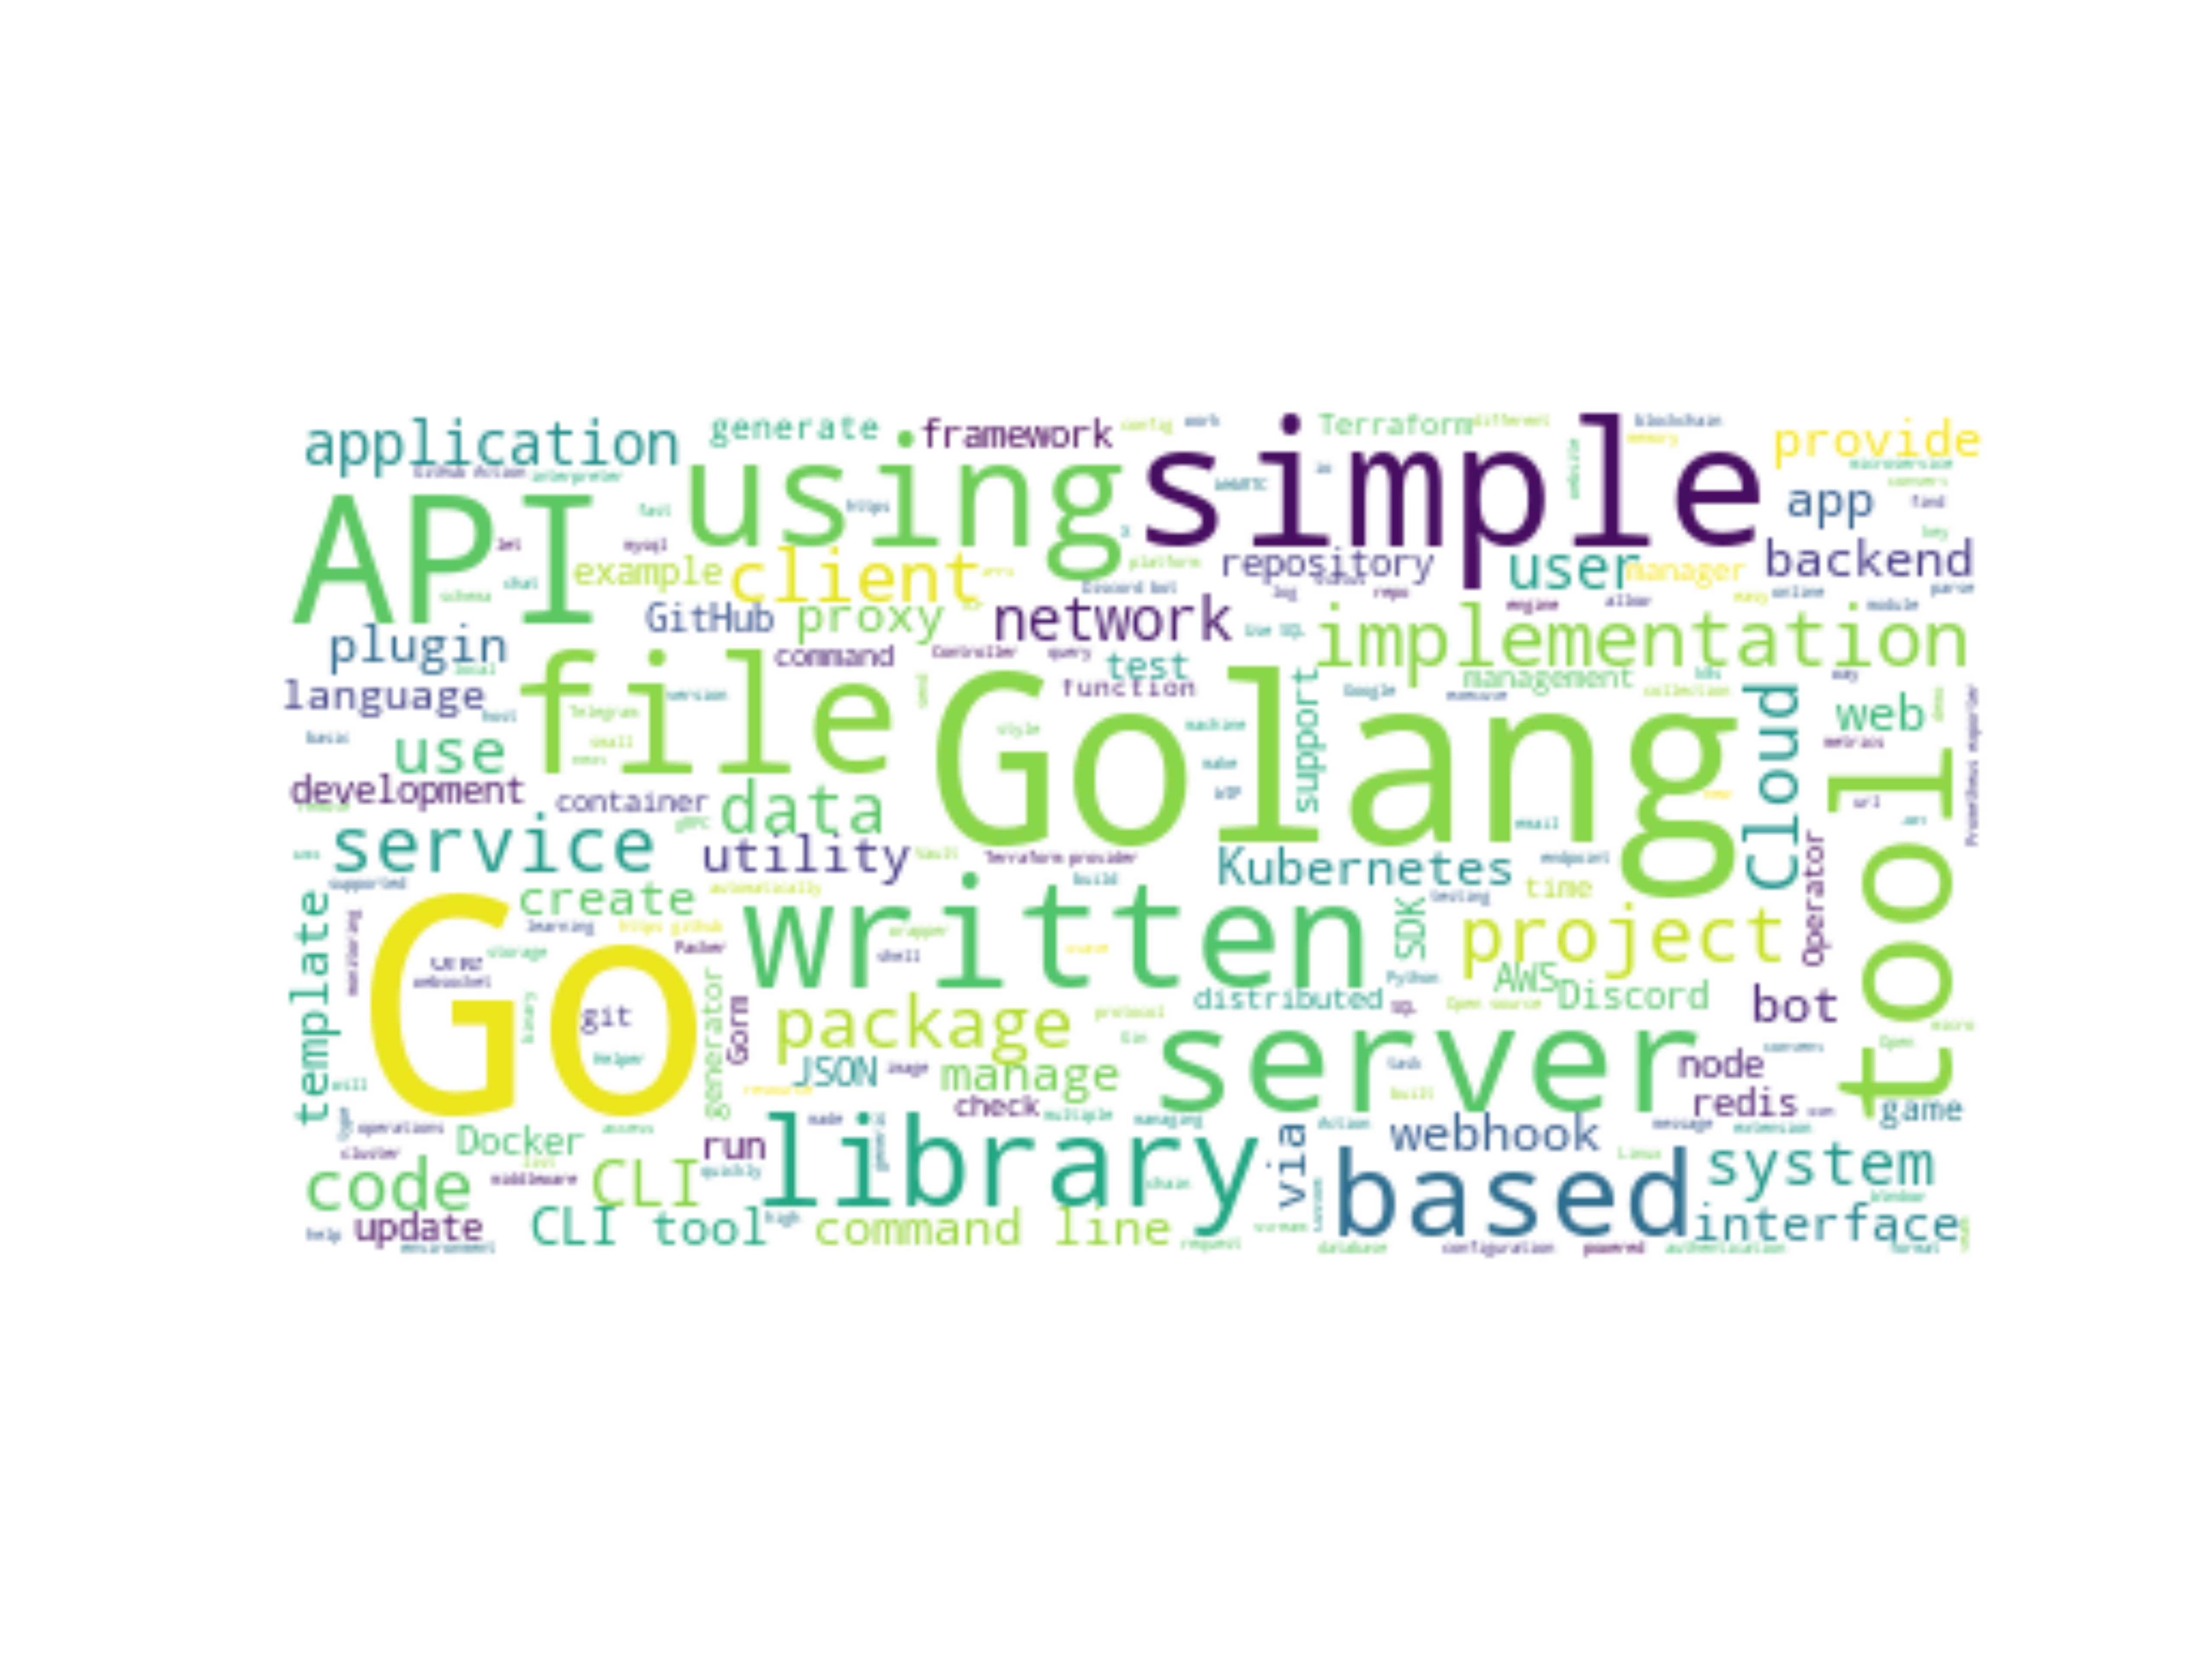
\includegraphics[scale=0.4]{result/wordcloud.png}
    \end{minipage}
}
\caption{figure title}
\end{figure}

\paragraph{} From the wordcloud pitures, we can see that developers using Go mainly use it for server and container development

 
\chapter{Conclution}
\paragraph{} According to the analysis of this report, we can come to the conclusion that with the development of the computer industry in recent years, Go language is also developing.
As more and more computer practitioners choose to recognize and use Go for their work, Go is worth further study.
\end{document}                          % The required last line